% Copyright 2004 by Till Tantau <tantau@users.sourceforge.net>.
%
% In principle, this file can be redistributed and/or modified under
% the terms of the GNU Public License, version 2.
%
% However, this file is supposed to be a template to be modified
% for your own needs. For this reason, if you use this file as a
% template and not specifically distribute it as part of a another
% package/program, I grant the extra permission to freely copy and
% modify this file as you see fit and even to delete this copyright
% notice. 

\documentclass{beamer}

% There are many different themes available for Beamer. A comprehensive
% list with examples is given here:
% http://deic.uab.es/~iblanes/beamer_gallery/index_by_theme.html
% You can uncomment the themes below if you would like to use a different
% one:
%\usetheme{AnnArbor}
%\usetheme{Antibes}
%\usetheme{Bergen}
%\usetheme{Berkeley}
%\usetheme{Berlin}
%\usetheme{Boadilla}
%\usetheme{boxes}
%\usetheme{CambridgeUS}
%\usetheme{Copenhagen}
%\usetheme{Darmstadt}
%\usetheme{default}
%\usetheme{Frankfurt}
%\usetheme{Goettingen}
%\usetheme{Hannover}
%\usetheme{Ilmenau}
%\usetheme{JuanLesPins}
%\usetheme{Luebeck}
\usetheme{Madrid}
%\usetheme{Malmoe}
%\usetheme{Marburg}
%\usetheme{Montpellier}
%\usetheme{PaloAlto}
%\usetheme{Pittsburgh}
%\usetheme{Rochester}
%\usetheme{Singapore}
%\usetheme{Szeged}
%\usetheme{Warsaw}

\usepackage{kotex}
\usepackage{braket}
\usepackage{array}
\usepackage{calc}
\usepackage{datetime}

\usepackage{listings}


\title{Lecture 1 : 강의 소개/집합과 함수}

% A subtitle is optional and this may be deleted
\subtitle{Fastcampus Math Camp}

\author{신승우}
% - Give the names in the same order as the appear in the paper.
% - Use the \inst{?} command only if the authors have different
%   affiliation.

% \institute[Universities of Somewhere and Elsewhere] % (optional, but mostly needed)
% {
  % \inst{1}%
  % Department of Computer Science\\
  % University of Somewhere
  % \and
  % \inst{2}%
  % Department of Theoretical Philosophy\\
  % University of Elsewhere}
% - Use the \inst command only if there are several affiliations.
% - Keep it simple, no one is interested in your street address.

% - Either use conference name or its abbreviation.
% - Not really informative to the audience, more for people (including
%   yourself) who are reading the slides online

\subject{Theoretical Computer Science}

% This is only inserted into the PDF information catalog. Can be left
% out. 

% If you have a file called "university-logo-filename.xxx", where xxx
% is a graphic format that can be processed by latex or pdflatex,
% resp., then you can add a logo as follows:

% \pgfdeclareimage[height=0.5cm]{university-logo}{university-logo-filename}
% \logo{\pgfuseimage{university-logo}}

% Delete this, if you do not want the table of contents to pop up at
% the beginning of each subsection:


\AtBeginSection[]
{
  \begin{frame}<beamer>{Outline}
    \tableofcontents[currentsection,hideallsubsections]
  \end{frame}
}

% Let's get started
\begin{document}

\begin{frame}
  \titlepage
\end{frame}

\begin{frame}{Outline}
  \tableofcontents[hideallsubsections]
  % You might wish to add the option [pausesections]
\end{frame}

% Section and subsections will appear in the presentation overview
% and table of contents.

\section{수업 소개}

\subsection{수업 목표} 

\begin{frame}{수업 목표} 

This lecture is about... 
\begin{itemize} 
\item 수학적 개념의 이해 
\item 기초적인 Computer Algebra System의 구현
\begin{itemize} 
\item symbolic implementation 
\item numerical implementation 
\end{itemize}
\item 학습한 수학적 개념의 응용법 살펴보기 
\end{itemize}

\end{frame}

\begin{frame}
This lecture is \textbf{NOT} about... 

\begin{itemize} 
\item 라이브러리 사용법 - We will re-invent the Wheel! 
\end{itemize}

본 수업에서 만들 것들은 대부분 sympy나 numpy에 포함되어 있습니다. 


\end{frame}

\subsection{수업 진행 방식} 

\begin{frame}{수업 진행 방식}
\begin{enumerate} 
\item 수학적 개념을 배운다. 
\item 구현 가능한 부분을 구현한다. \footnote{구현 불가능한 부분을 정확하게 구분하고 싶으면, 나중에 Computable Analysis 같은 부분을 공부하면 됩니다. 여기서는 다루지 않습니다. }
\item 구현한 부분을 일부 사용하고, 기존 라이브러리(numpy 등)의 도움을 받아서 실제 공학적 문제를 해결해 본다. 
\end{enumerate}

모든 구현 결과와 수업자료는 깃헙에 올라갑니다. 
\end{frame}

\begin{frame}{구현에서의 이슈들}
본격적으로 수업 전에, 구현에서 많이 있을 이슈들을 짚고 넘어갑니다. 
\begin{itemize}
\item 무한을 다루는 법 
\begin{itemize} 
\item 무한집합 
\item 실수 / 무리수 
\end{itemize}
\item symbolic한 식을 다루는 법 
\end{itemize}
\end{frame}

\begin{frame}{Handling Infinite} 

기본적으로 컴퓨터나 우리의 시간은 유한하므로, 무한을 다루는 것은 불가능합니다. 따라서 우리는 무한을 다음과 같은 근사적인 형태로 다룹니다. 

\begin{itemize}
\item lazy evaluation 사용 : 파이썬에서 제공하므로 명시적으로 구현할 필요는 없음
\item semi-decidable loop 사용 
\item 최대 수를 정해놓고 유한으로 근사하기 
\end{itemize}

\end{frame}

\section{집합} 

\subsection{집합의 정의} 

\begin{frame}{집합의 정의}

집합은 다음과 같이 정의됩니다. 

\begin{block}{집합}
특정 조건에 맞는 원소들의 모임. 임의의 한 원소가 그 모임에 속하는지를 알 수 있고, 그 모임에 속하는 임의의 두 원소가 다른가 같은가를 구별할 수 있는 명확한 표준이 있는 것을 이른다. 
\end{block}

여기서 집합을 이루는 것은 두 가지임을 알 수 있습니다. 

\begin{itemize}
\item 임의의 한 원소가 그 모임에 속하는지를 알 수 있고
\item 그 모임에 속하는 임의의 두 원소가 다른가 같은가를 구별할 수 있는 명확한 표준
\end{itemize}

이를 조금 더 구현 가능한 말로 바꿔보겠습니다. 

\end{frame}

\begin{frame}{집합의 정의}
\begin{itemize}
\item 임의의 원소가 그 모임에 속하는지 판단하는 함수 : isinstance 함수
\item 두 원소가 같은지 판단하는 함수 : \_\_eq\_\_ 함수 
\end{itemize}

위에서 나와있듯이, 이 둘은 파이썬의 클래스에서 이미 구현되어 있습니다. 즉, 우리는 파이썬의 클래스를 집합으로 간주할 수 있습니다. 
본 수업에서는 숫자의 집합만을 고려할 예정이므로, 두번째 함수는 구현하지 않을 것입니다. 
\end{frame}

\subsection{집합의 연산} 
\begin{frame}{집합의 연산}
\begin{itemize}
\item 집합의 크기 $|A|$
\item 합집합 $A \cup B$
\item 교집합 $A \cap B$
\item 차집합 $A-B$
\item 데카르트 곱 $A \times B$
\end{itemize}
\end{frame}

\subsection{집합의 종류} 
\begin{frame}{집합의 종류}

여기서는 집합의 크기\footnote{무한집합의 경우에는 크기보다는 농도라는 표현을 씁니다.}에 따른 분류와, 집합의 순서 여부에 따른 분류를 배웁니다. 
\begin{itemize}
\item 크기에 따라 
\begin{itemize} 
\item 유한집합 
\item 가산집합
\item 비가산집합 
\end{itemize}

\item 순서 여부에 따라 
\begin{itemize}
\item Orderless Set 
\item Partially Ordered Set 
\item Ordered Set
\end{itemize}
\end{itemize}
\end{frame}



\begin{frame}{가산집합}
가산집합은 그 수를 셀 수 있는 집합을 말합니다. 여기서 센다는 것은, 집합의 각 원소에 일련번호를 붙일 수 있다는 말과 같습니다. 
\\
센다는 것을 프로그래밍에서 생각해보면, iterator\footnote{iterator를 모르시는 분은 DB 커서를 생각하셔도 됩니다.}의 개념과 흡사하다는 것을 알 수 있습니다. 즉, 센다는 행위를 iterator에서 next() 함수를 호출하는 것과 같이 생각할 수 있습니다. \\
엄밀하게는, 가산집합은 자연수 집합과 일대일대응이 가능한 집합을 말합니다. 
\end{frame}


\begin{frame}{가산집합의 예시}
\begin{itemize}
\item 자연수
\item 짝수/홀수
\item 정수
\item 유리수 
\end{itemize}
\end{frame}

\begin{frame}{비가산집합}

그렇다면, 셀 수 없는 집합이 있을까요? 대표적으로 실수는 셀 수 없습니다. 
\begin{itemize}
\item 실수
\end{itemize}
실수는 전산상으로 완벽하게 구현이 불가능함을 보일 수 있습니다. 따라서 여기서는 실수를 구현하지 않고, 그냥 유리수로 실수를 대체하여 사용합니다. 
\end{frame}

\begin{frame}{Ordered Set}
일반적으로 집합은 순서가 없습니다. 하지만, 집합에 순서를 부여하는 것은 가능합니다. 예를 들어서, 어떤 사전에 있는 단어들의 집합을 생각해 보면, 집합의 두 가지 조건을 만족하면서 동시에 순서도 있습니다. 

특히, 사전에 있는 단어는 모든 단어가 다 순서를 가지고 있습니다. 즉, 임의의 두 단어간에 사전에서 더 앞에 오는 단어가 있습니다. 이런 경우 Totally Ordered Set이라고 합니다. 

반면, 항상 모든 원소간에 항상 순서가 잘 정의되는 것은 아닙니다. 이런 경우를 Partially Ordered Set이라고 합니다. 
\end{frame}



% \begin{frame}{}
% \begin{itemize}
% \end{itemize}
% \end{frame}


\begin{frame}{집합의 구현}
이제 위에서 배운 개념들을 구현해 보겠습니다. 
\begin{itemize}
\item 집합과 그 연산
\item 유한집합/가산집합 
\item Ordered/Partially Ordered Set 
\item 자연수/유리수
\end{itemize}
\end{frame}

\section{함수} 

\begin{frame}{함수}
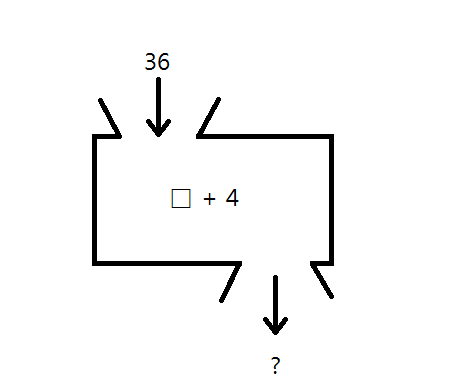
\includegraphics[height=\textheight]{function}\footnote{출처 : http://itguru.tistory.com/26}
\end{frame}

\subsection{함수의 정의}
\begin{frame}{함수의 정의}

함수는 다음과 같이 정의됩니다. 

\begin{block}{함수}
함수는 정의역(X, domain), 공역(Y, codomain), 그리고 대응관계(f, function)로 정의됩니다. 
\end{block}

정의역과 공역은 집합이며, 대응관계는 정의역의 한 원소를 공역의 한 원소로 대응시킵니다. 이 때, 다음의 공역의 부분집합을 치역이라고 하고 다음과 같이 씁니다. 
$f(X) = \{y|\forall x \in X, y=f(x)\}$
\end{frame}

\begin{frame}{함수의 정의}
위 내용을 프로그래밍적으로 생각해 보면 
\begin{itemize}
\item 정의역 : 함수의 input argument의 type
\item 치역 : 함수의 return value의 type 
\item 대응관계 : 함수 내부 body 
\end{itemize}
로 볼 수 있습니다. 예를 들어서 자바의 함수 헤더의 경우, \\
public int methodName(int a, int b) \\
으로 쓰이는데, 이는 정확하게 함수의 수학적 정의와 일치함을 볼 수 있습니다. 
\end{frame}

\subsection{함수의 종류}
\begin{frame}{함수의 종류}
\begin{itemize}
\item 단사함수 : 공역과 치역이 같은 함수
\item 전사함수 : 정의역의 각자 다른 원소를 공역의 각자 다른 원소로 대응시키는 함수
\item 전단사함수 : 단사이면서 전사인 함수
\end{itemize}

\end{frame}

\subsection{합성함수}
\begin{frame}{합성함수의 정의}
두 함수 f,g에 대하여 합성함수는 다음과 같이 정의됩니다. 
\begin{block}{합성함수}
합성함수 $f \bullet g$는 f(g(x))로 정의됩니다. 
\end{block}
이 때 g의 공역과, f의 정의역이 일치해야 두 함수를 합성할 수 있습니다. 프로그래밍으로 비유하자면, TypeError가 안 나게 해야 하는 것과 같습니다. 

\end{frame}

\subsection{역함수}
\begin{frame}{역함수}
함수 f에 대하여 역함수는 다음과 같이 정의됩니다. 
\begin{block}{역함수}
함수 f의 역함수 $f^{-1}$는 $\forall x \in X, f(f^{-1}(x)) = x$ 를 만족하는 함수를 말한다. 
\end{block}
\end{frame}

\begin{frame}{함수의 구현}
이제 위에서 배운 함수의 개념들을 구현해 보겠습니다. 
\begin{itemize}
\item 함수 
\item 합성함수
\item 역함수 
\end{itemize}
\end{frame}

\section{다양한 함수와 그 성질} 

\subsection{다항함수}

\begin{frame}{다항함수}
$a_nx^n + a_{n-1}x^{n-1} + ... + a_1 x^1 + a_0 = \sum^{n}_{i=0} a_i x^i$
와 같은 함수를 다항함수라 하고, n차함수라고도 한다. 
\end{frame}

\subsection{삼각함수} 
\begin{frame}{삼각함수의 정의}
\begin{centering}
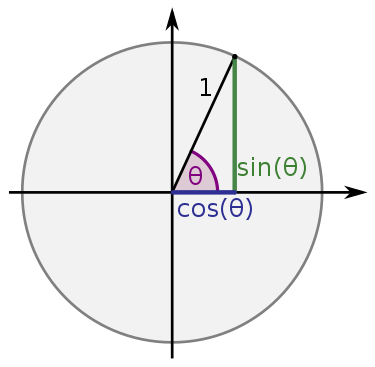
\includegraphics[height = 0.8\textheight]{trigo}
\end{centering}
\end{frame}

\begin{frame}{Sine 함수}
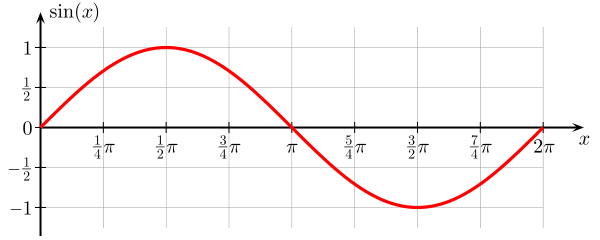
\includegraphics[width=\textwidth]{sin}
\end{frame}

\begin{frame}{Cosine 함수}
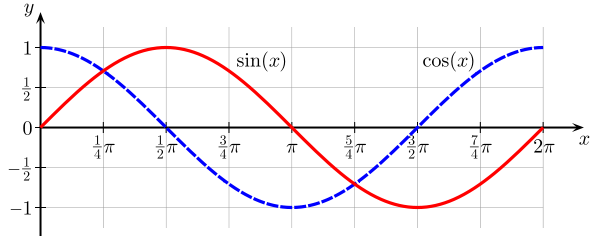
\includegraphics[width=\textwidth]{cos}
\end{frame}

\begin{frame}{삼각함수의 성질}
\begin{itemize}
\item $tan(x) = \frac{sin(x)}{cos(x)}$ \footnote{tan 함수의 정의}
\item $sin^2(x) + cos^2(x) = 1$
\end{itemize}
\end{frame}

\begin{frame}{삼각함수의 성질}
세 변의 길이가 a,b,c이고 각 변을 바라보는 각이 각각 $\alpha, \beta, \gamma$인 넓이가 S인 삼각형에 대해서 다음이 성립합니다. 
\begin{itemize}
\item $S = \frac{1}{2} bc sin(\alpha)$
\item $c^2 = a^2 + b^2 - 2ab cos(\gamma)$
\end{itemize}
\end{frame}

\begin{frame}{삼각함수의 합차공식}

\begin{itemize}
\item $sin(x+y) = sin(x)cos(y) + sin(y)cos(x)$
\item $cos(x+y) = cos(x)cos(y) - sin(x)sin(y)$
\item $tan(x+y) = \frac{tan(x)tan(y)}{1-tan(x)tan(y)}$
\end{itemize}
\end{frame}




\subsection{지수/로그함수} 

\begin{frame}{지수법칙}
정수 n,m에 대해서 다음이 성립합니다. 

\begin{itemize}
\item $x^n x^m = x^{n+m}$
\item $\frac{x^n}{x^m} = x^{n-m}$
\item $(x^n)^m = x^{nm}$
\end{itemize}
\end{frame}


\begin{frame}{지수함수}
지수법칙을 실수로 연장하여 생각하면, 다음과 같은 함수를 생각할 수 있습니다. 
\begin{block}{지수함수}
양의\footnote{음의 경우는 다루지 않습니다.} 상수 a에 대해서, 다음과 같은 함수를 지수함수라고 합니다. $f(x) = a^x$
\end{block}
\end{frame}

\begin{frame}{지수함수}
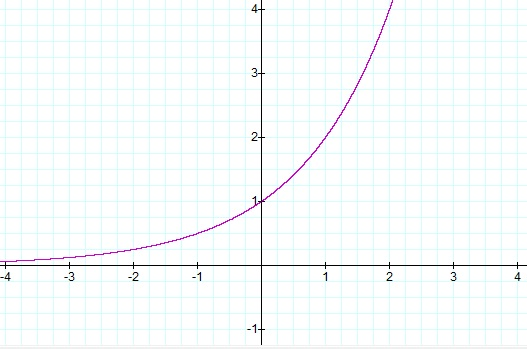
\includegraphics[width=\textwidth]{exp}
\end{frame}

\begin{frame}{로그함수} 
\begin{block}{로그함수}
양의\footnote{음의 경우는 다루지 않습니다.} 상수 a에 대해서, 다음과 같은 함수를 지수함수라고 합니다. $y = log_{a} x$ 이면 $ x = y^a$
\end{block}
로그함수와 지수함수는 역함수 관계입니다. 

\end{frame}

\begin{frame}{로그함수의 성질} 
\begin{itemize} 
\item $log MN = log M + log N$
\item $log (M/N) = log M - log N$
\item $log M^k = k log M $
\end{itemize}
\end{frame}

\end{document}


